\appendix
\addcontentsline{toc}{chapter}{Appendices}
\startcontents
\startlist[appendix]{lof}
\startlist[appendix]{lot}
\printcontents{atoc}{0}{\chapter*{Appendices}}
\begingroup
\let\clearpage\relax
\singlespacing
\printlist[appendix]{lof}{}{\chapter*{List of Figures}}
\printlist[appendix]{lot}{}{\chapter*{List of Tables}}
\endgroup

\chapter{Establishment of methods to assess genome-wide chromatin accessibility}
\label{app:optimisation}

\begin{figure}[htbp]
\centering
\begin{subfigure}{0.70\textwidth}
\centering
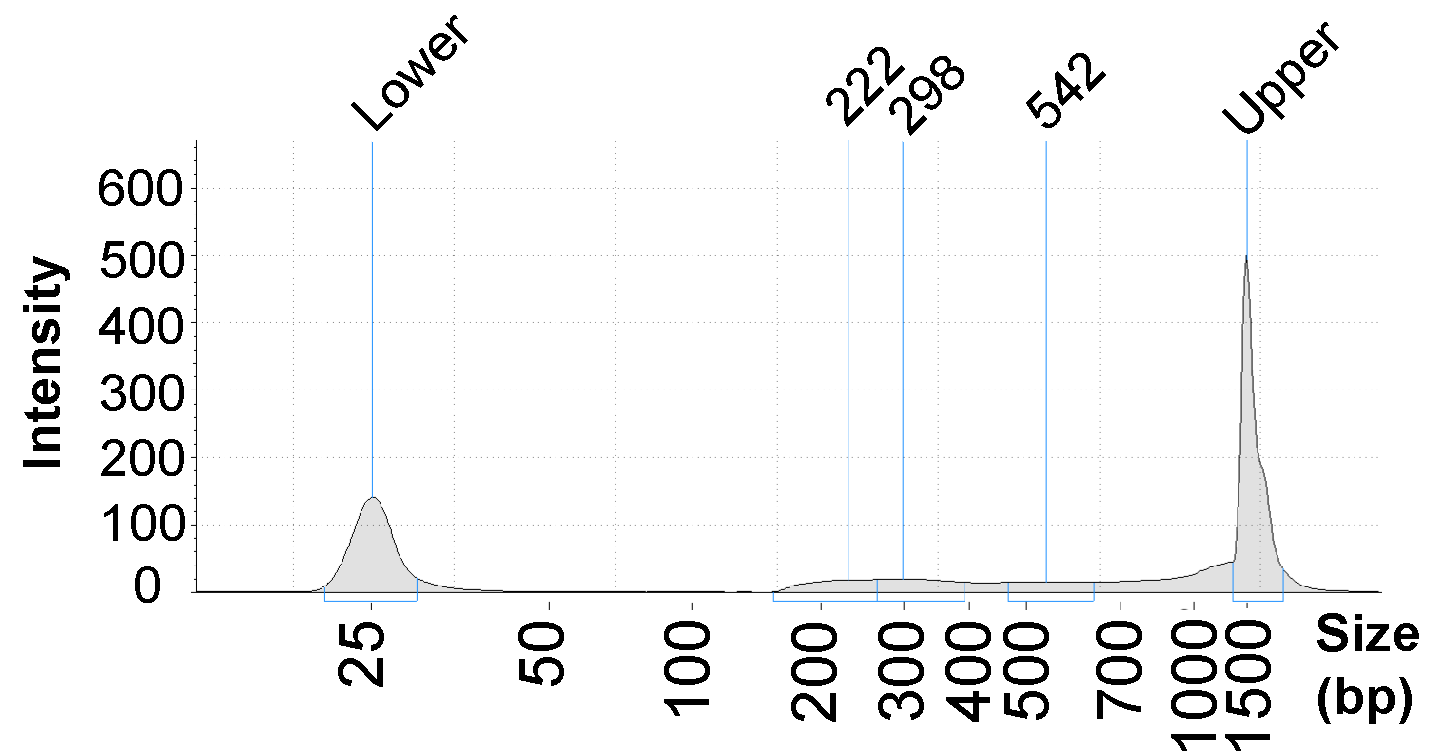
\includegraphics[width=\textwidth]{./Appendix/pdfs/Chapter3/FAST_ATAC_skin_tapestation_C1}
\caption{\textbf{}}
% The percentage sign indicated that the other subfig goes side by side
\end{subfigure}
\begin{subfigure}{0.70\textwidth}
\centering
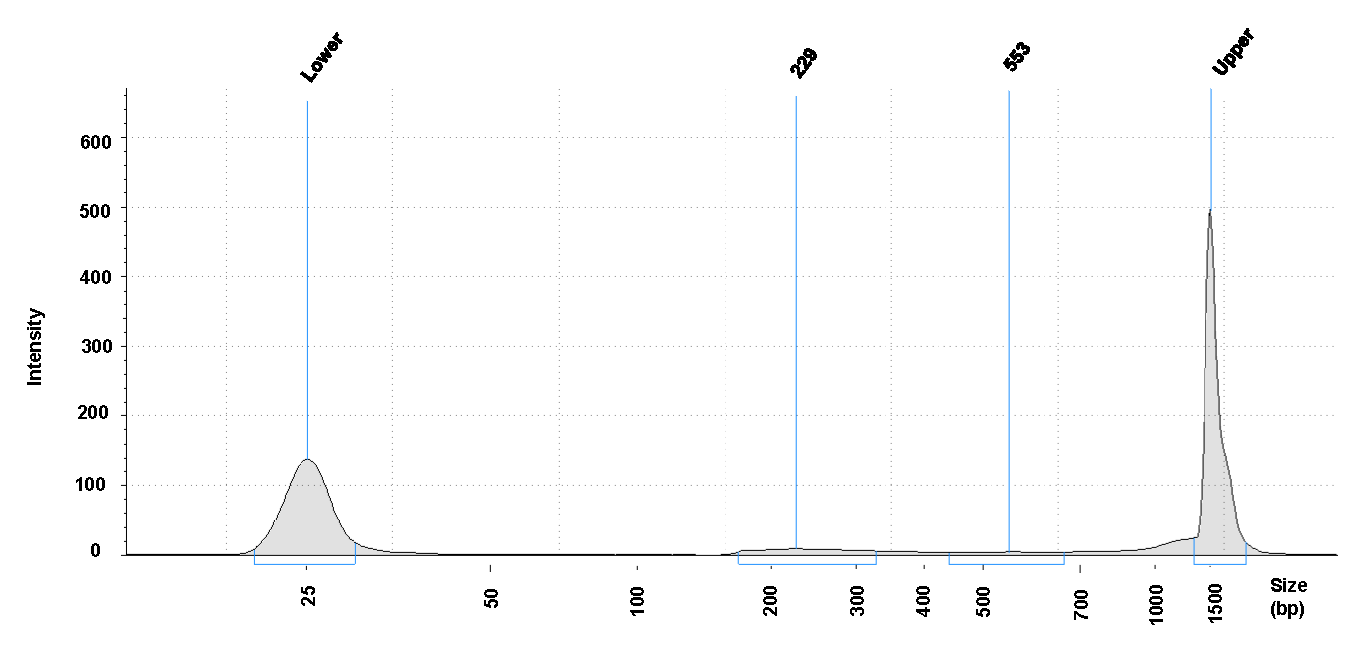
\includegraphics[width=\textwidth]{./Appendix/pdfs/Chapter3/FAST_ATAC_skin_tapestation_C3}
\caption{\textbf{}}
\end{subfigure}
\begin{subfigure}{0.70\textwidth}
\centering
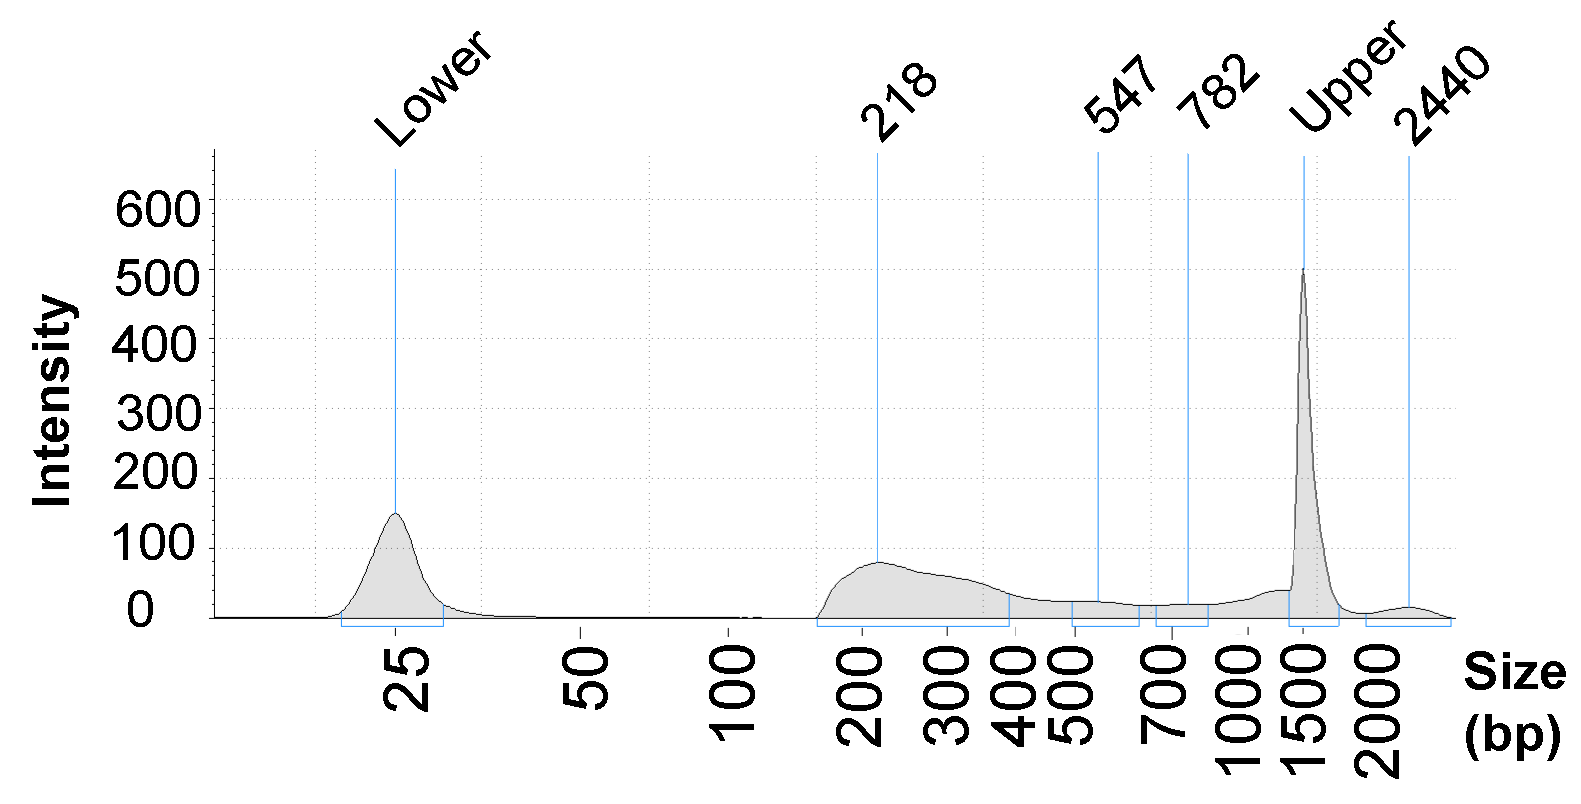
\includegraphics[width=\textwidth]{./Appendix/pdfs/Chapter3/FAST_ATAC_skin_tapestation_C4}
\caption{\textbf{}} % to add text to the figure name
\end{subfigure}
\begin{subfigure}{0.70\textwidth}
\centering
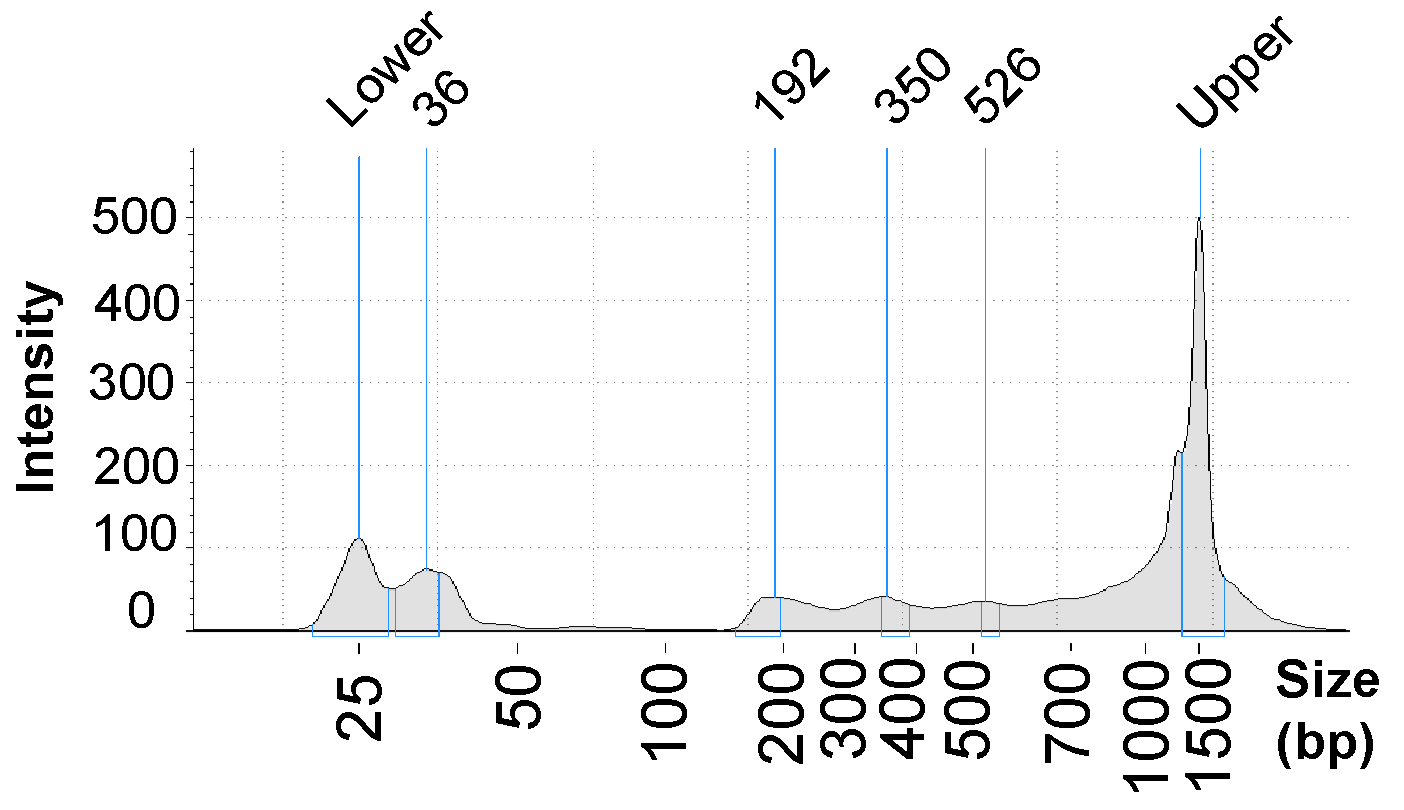
\includegraphics[width=\textwidth]{./Appendix/pdfs/Chapter3/Omni_ATAC_NHEK_Rep1_tapestation}
\caption{\textbf{}} % to add text to the figure name
\end{subfigure}
\hfill
\caption[FAST-ATAC and Omni-ATAC NHEK tapestation profiles.]{\textbf{FAST-ATAC and Omni-ATAC NHEK tapestation profiles.} \\
}
\label{fig:NHEK_tapestation}
\end{figure}



\begin{figure}[htbp]
\centering
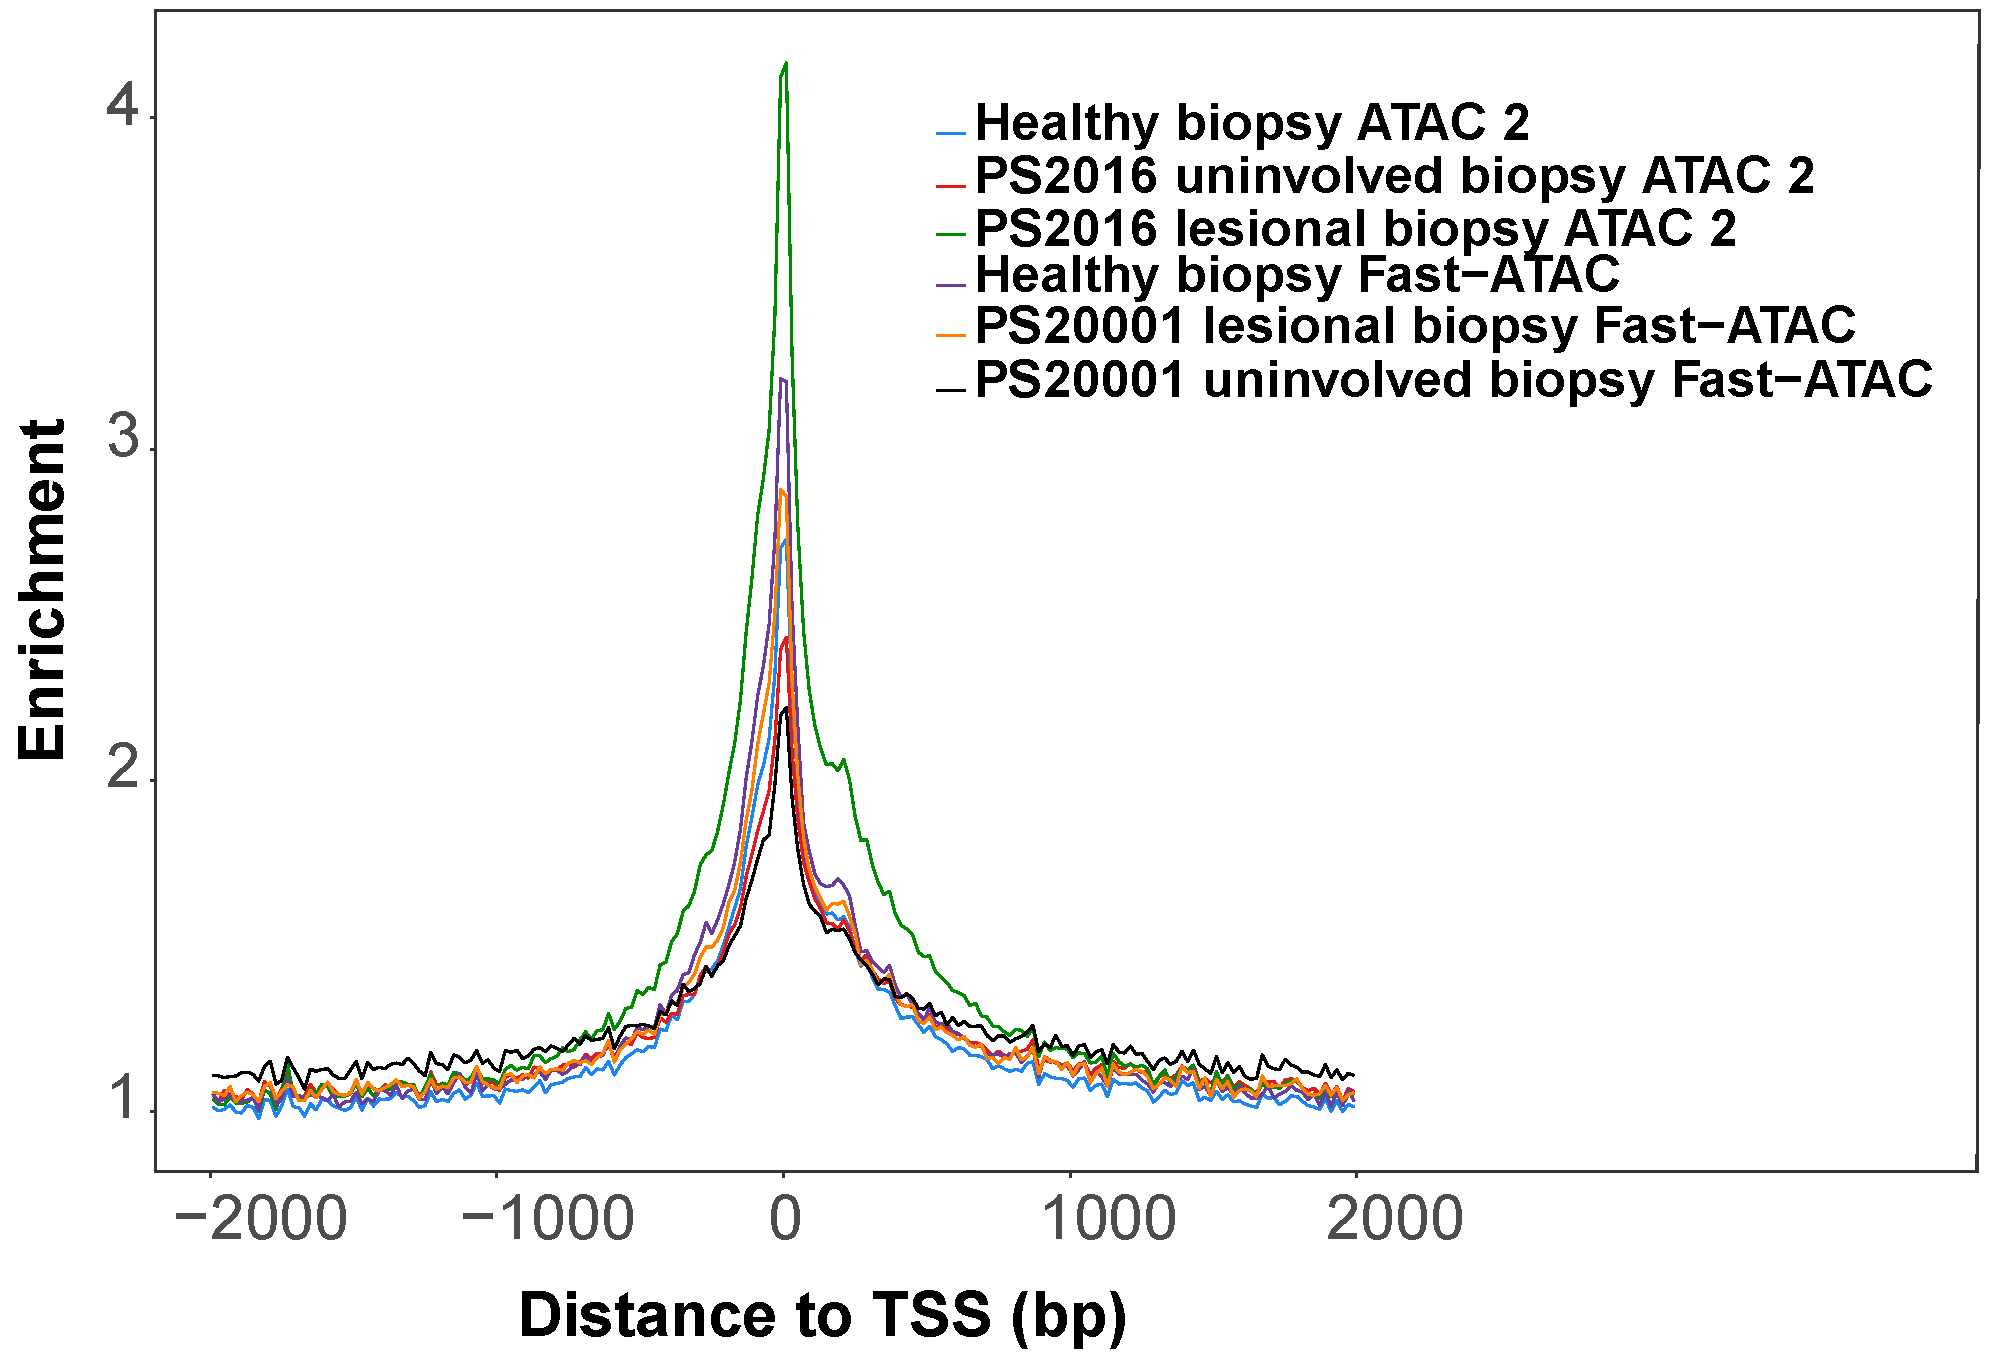
\includegraphics[width=0.8\textwidth]{./Appendix/pdfs/Chapter3/ATAC_skin_biopsy_samples_all_methods_TSS_enrichment_supplementary}
\caption[Assessment of TSS enrichment from ATAC-seq and FAST-ATAC in healthy and psoriasis skin biopsies samples.]{\textbf{Assessment of TSS enrichment from ATAC-seq and FAST-ATAC in healthy and psoriasis skin biopsies samples.}  }
\label{fig:TSS_skin_biopsies}
\end{figure}



\chapter{Cross-tissue comparison analysis in PsA}
\label{app:cross_tissue_PsA}

\bigskip
\begin{figure}[H]
\centering
\begin{subfigure}[b]{0.45\textwidth}
\centering 
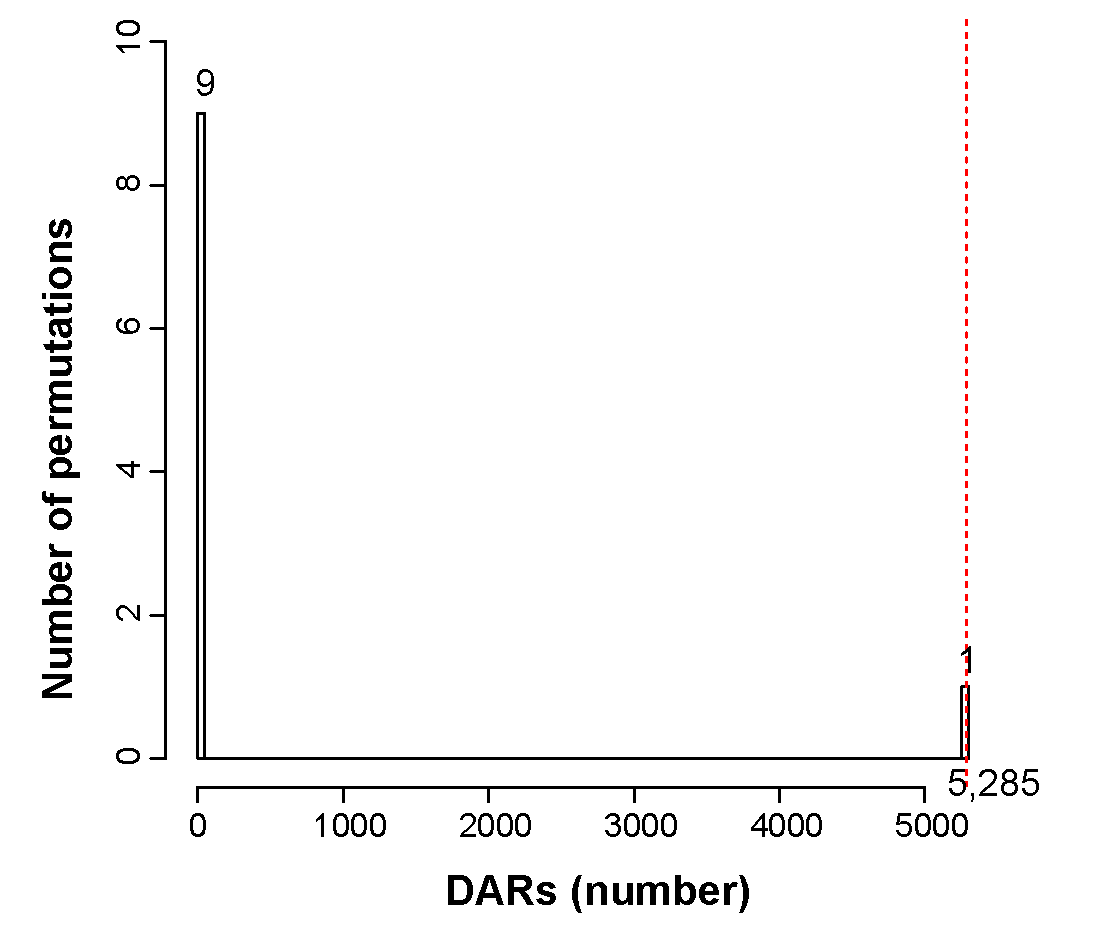
\includegraphics[width=\textwidth]{./Appendix/pdfs/Chapter5/ATAC_PsA_CD14_permutation_analysis}
\caption{}
\end{subfigure}
~
\begin{subfigure}[b]{0.45\textwidth}
\centering 
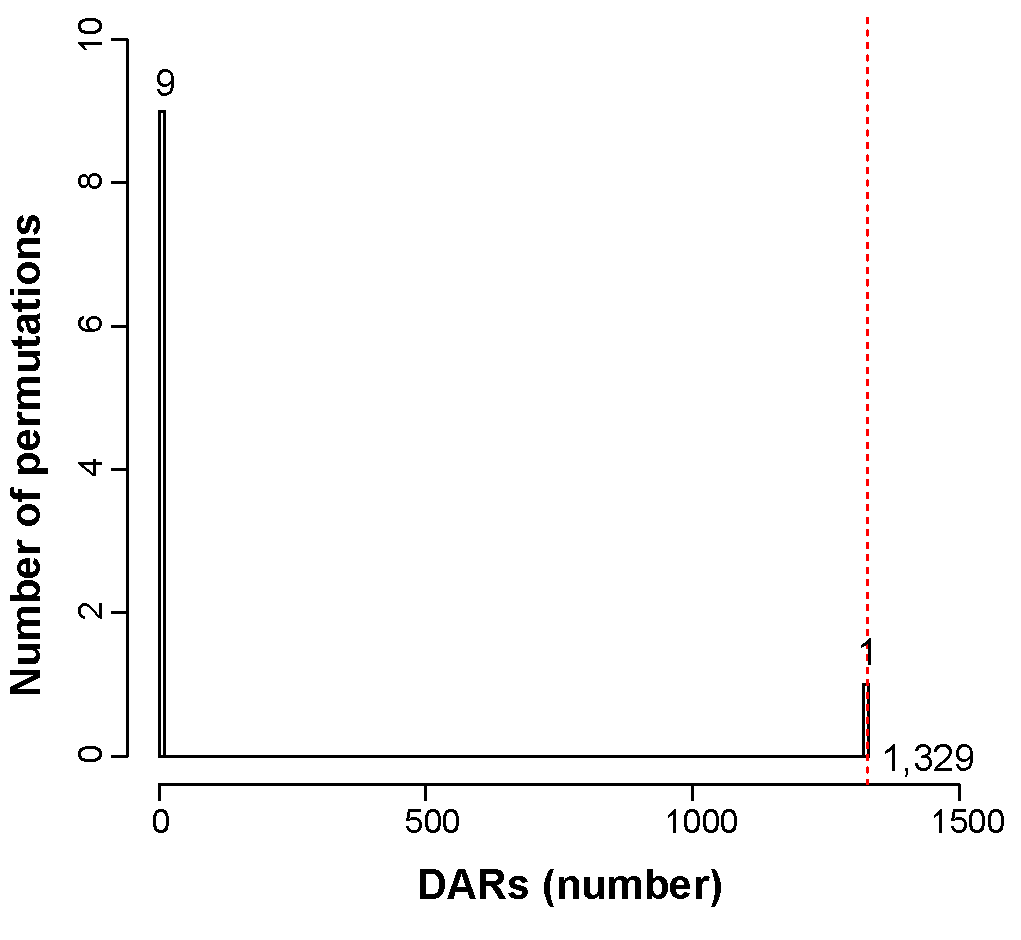
\includegraphics[width=\textwidth]{./Appendix/pdfs/Chapter5/ATAC_PsA_CD4_permutation_analysis}
\caption{}
\end{subfigure}
~
\begin{subfigure}[b]{0.45\textwidth} 
%the [b] prevents offset in subcaptions
\centering
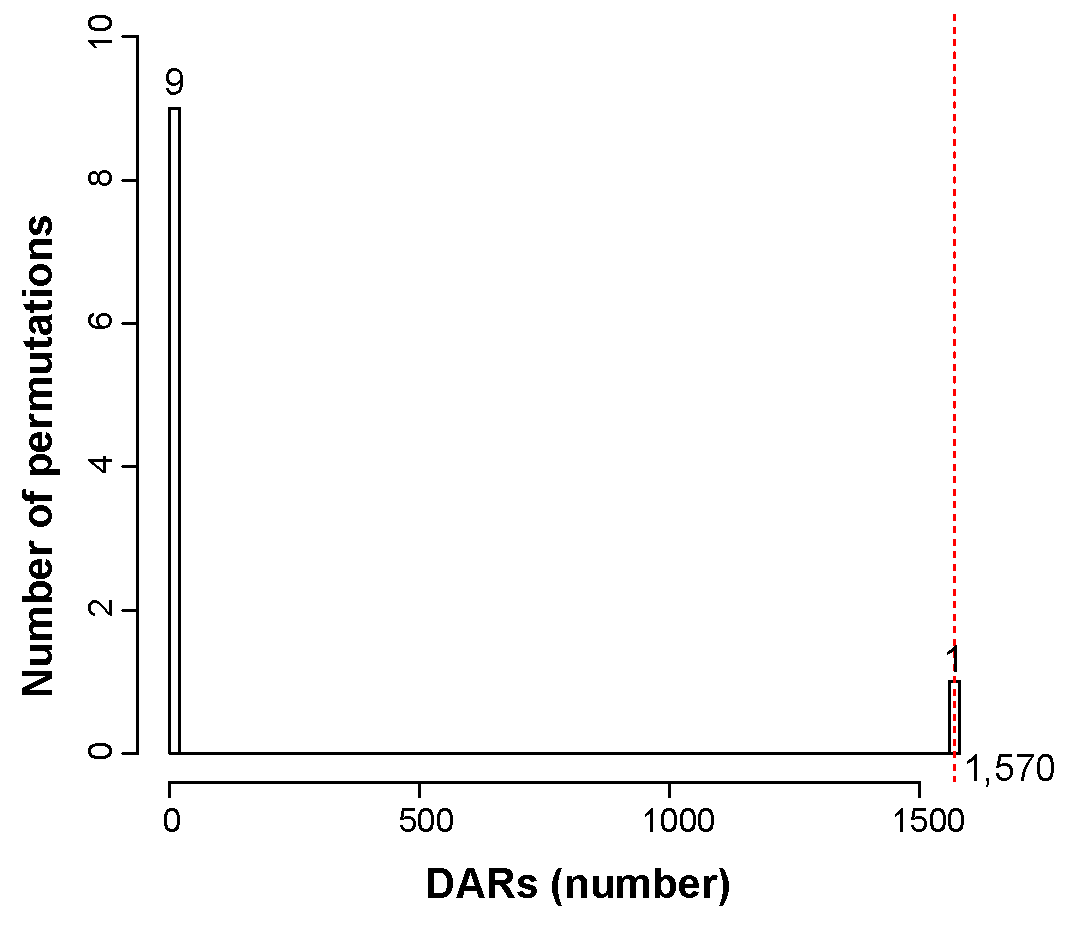
\includegraphics[width=\textwidth]{./Appendix/pdfs/Chapter5/ATAC_PsA_CD8_permutation_analysis}%
\caption{}
\end{subfigure}
\begin{subfigure}[b]{0.45\textwidth} 
%the [b] prevents offset in subcaptions
\centering
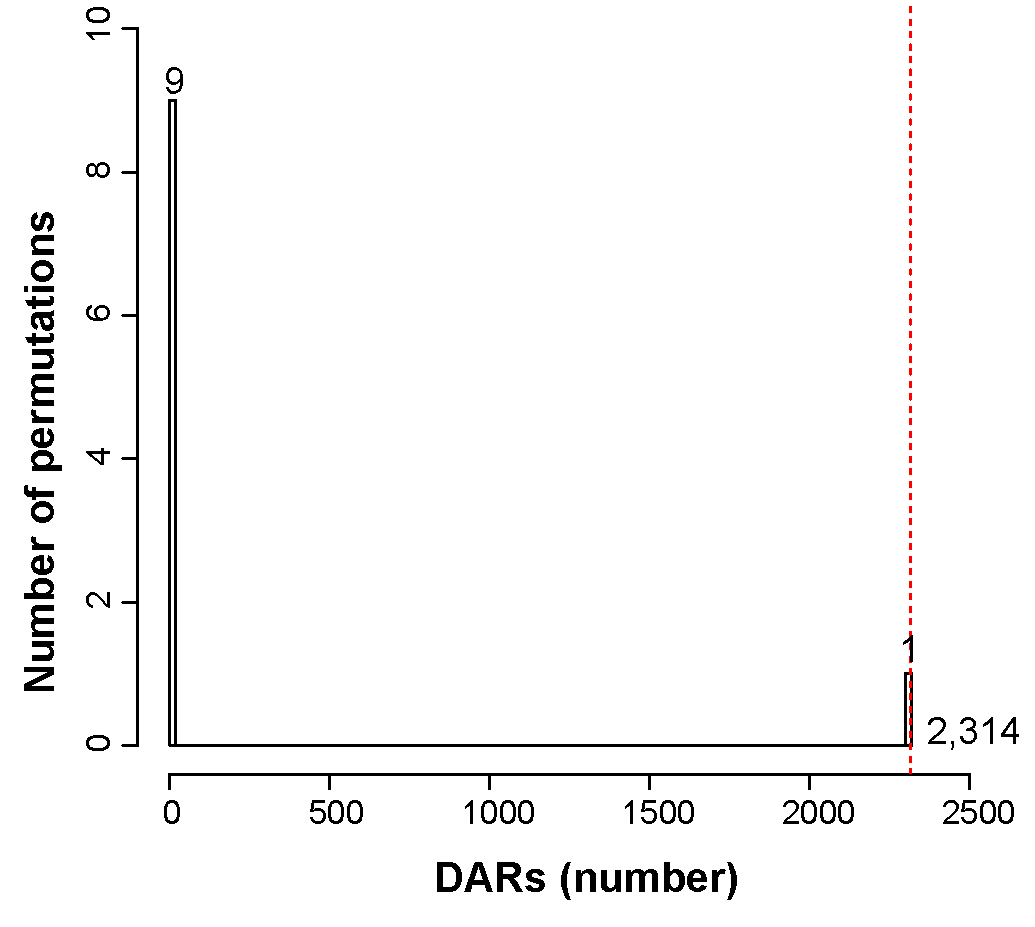
\includegraphics[width=\textwidth]{./Appendix/pdfs/Chapter5/ATAC_PsA_NK_permutation_analysis}%
\caption{}
\end{subfigure}
\caption[Permutation analysis SF vs PB in CD14$^+$,CD4m$^+$,CD8m$^+$ and NK.]{\textbf{Permutation analysis SF vs PB in CD14$^+$,CD4m$^+$,CD8m$^+$ and NK}. }
\label{figure:PsA_perm_analysis}
\end{figure}